\documentclass{beamer}
\let\vec\mathbf
\mode<presentation>
\usepackage{amsmath}
\usepackage{amssymb}
%\usepackage{advdate}
\usepackage{adjustbox}
%\usepackage{subcaption}
\usepackage{enumitem}
\usepackage{multicol}
\usepackage{mathtools}
\usepackage{listings}
\usepackage{url}
\usetheme{Boadilla}
\usecolortheme{lily}
\setbeamertemplate{footline}
{
  \leavevmode%
  \hbox{%
  \begin{beamercolorbox}[wd=\paperwidth,ht=2.25ex,dp=1ex,right]{author in head/foot}%
    \insertframenumber{} / \inserttotalframenumber\hspace*{2ex} 
  \end{beamercolorbox}}%
  \vskip0pt%
}
\setbeamertemplate{navigation symbols}{}
\providecommand{\nCr}[2]{\,^{#1}C_{#2}} % nCr
\providecommand{\nPr}[2]{\,^{#1}P_{#2}} % nPr
\providecommand{\mbf}{\mathbf}
\providecommand{\pr}[1]{\ensuremath{\Pr\left(#1\right)}}
\providecommand{\qfunc}[1]{\ensuremath{Q\left(#1\right)}}
\providecommand{\sbrak}[1]{\ensuremath{{}\left[#1\right]}}
\providecommand{\lsbrak}[1]{\ensuremath{{}\left[#1\right.}}
\providecommand{\rsbrak}[1]{\ensuremath{{}\left.#1\right]}}
\providecommand{\brak}[1]{\ensuremath{\left(#1\right)}}
\providecommand{\lbrak}[1]{\ensuremath{\left(#1\right.}}
\providecommand{\rbrak}[1]{\ensuremath{\left.#1\right)}}
\providecommand{\cbrak}[1]{\ensuremath{\left\{#1\right\}}}
\providecommand{\lcbrak}[1]{\ensuremath{\left\{#1\right.}}
\providecommand{\rcbrak}[1]{\ensuremath{\left.#1\right\}}}
\theoremstyle{remark}
\newtheorem{rem}{Remark}
\newcommand{\sgn}{\mathop{\mathrm{sgn}}}

\providecommand{\res}[1]{\Res\displaylimits_{#1}} 
\providecommand{\norm}[1]{\lVert#1\rVert}
\providecommand{\mtx}[1]{\mathbf{#1}}

\providecommand{\fourier}{\overset{\mathcal{F}}{ \rightleftharpoons}}
%\providecommand{\hilbert}{\overset{\mathcal{H}}{ \rightleftharpoons}}
\providecommand{\system}{\overset{\mathcal{H}}{ \longleftrightarrow}}
	%\newcommand{\solution}[2]{\textbf{Solution:}{#1}}
%\newcommand{\solution}{\noindent \textbf{Solution: }}
\providecommand{\dec}[2]{\ensuremath{\overset{#1}{\underset{#2}{\gtrless}}}}
\newcommand{\myvec}[1]{\ensuremath{\begin{pmatrix}#1\end{pmatrix}}}

\title{Matrices in Geometry - 1.5.25}
\author{EE25BTECH11037  Divyansh}
\date{Aug, 2025}

\begin{document}

\maketitle


\begin{frame}
\tableofcontents
\end{frame}
\section{Problem}
\begin{frame}
\frametitle{Problem Statement}
In what ratio does the point $\vec{R}=\myvec{\frac{24}{11} \\ y}$ divide the line segment joining the points $\vec{P}=\myvec{2 \\ -2}$ and $\vec{Q}=\myvec{3 \\ 7}$? Also find the value of y.
\end{frame}

\section{Solution}
\begin{frame}{Solution}
   $\vec{P}=\myvec{2\\-2}$, $\vec{Q}=\myvec{3\\7}$ and a point $\vec{R}=  \myvec{\frac{24}{11} \\ y}$ on $PQ$. \\
   Let $R$ divide $PQ$ internally in the ratio $k:1$.\\
   Therefore, they are defined to be collinear if rank of the collinearity matrix is 1
   \begin{align*}
    \text{Collinearity matrix is }\myvec{\vec{P}- \vec{R} & \vec{Q}-\vec{R}}^{\top}=1\\
    \vec{P}-\vec{R}=\myvec{\dfrac{-2}{11} \\ -y-2}\\
    \vec{Q}-\vec{R}=\myvec{\dfrac{9}{11} \\ 7-y}\\
    \implies \text{rank}\myvec{\dfrac{-2}{11} & -y-2 \\ \dfrac{9}{11} & 7-y} = 1
\end{align*}
\end{frame}



\begin{frame}{Solution}
\begin{align*}
 \myvec{\frac{-2}{11} & -2-y \\ \frac{9}{11} & 7-y}\overset{R_2 \rightarrow R_2 + \frac{9}{2}R_1}{\longrightarrow} \myvec{\frac{-2}{11} & -2-y \\ 0 & \dfrac{-11-4y}{2}}\\
 \end{align*}
for rank of this matrix to be 1, all the elements in the lower row have to be zero
\begin{align*}
    \therefore -11-4y=0 \implies
    y=\dfrac{-4}{11}  
\end{align*}

We know that $k$ is the ratio in which $\vec{R}$ divides $\vec{P}$ and $\vec{Q}$,
\begin{align*}
    \vec{R}=\dfrac{k\vec{Q}+\vec{P}}{1+k}\\
   k\brak{\vec{R}-\vec{Q}}&= \vec{P}-\vec{R}\\
\end{align*}
\end{frame}

\begin{frame}{Solution}
   \begin{align*}
    \implies k =\dfrac{\brak{\vec{P}-\vec{R}}^{\top}\brak{\vec{R}-\vec{Q}}}{\norm{\vec{R}-\vec{Q}}^2}\\
   \brak{\vec{P}-\vec{R}}^{\top}=\myvec{\frac{-2}{11} & \frac{-18}{11}}\\
   \brak{\vec{R}-\vec{Q}}=\myvec{\frac{-9}{11} \\ \frac{-81}{11}}\\
   \norm{\vec{R}-\vec{Q}}^2=\myvec{\vec{R}-\vec{Q}}^{\top} \myvec{\vec{R}-\vec{Q}}\\=\myvec{\frac{-9}{11} & \frac{-81}{11}}\myvec{\frac{-9}{11} \\ \frac{-81}{11}}=\frac{81}{121} + \frac{6561}{121}=\frac{6642}{121}\\
   \end{align*}


\end{frame}
\begin{frame}{Solution}
    \begin{align*}
     \therefore k=\dfrac{\myvec{\frac{-2}{11} & \frac{-18}{11}}\myvec{\frac{-9}{11} \\ \frac{-81}{11}}}{\frac{6642}{121}}\\
        \implies k=\dfrac{\dfrac{18}{121} + \dfrac{1458}{121}}{\dfrac{6642}{121}}\\ \\ 
   \implies k=\dfrac{1476}{6624}=\dfrac{2}{9}
    \end{align*}
\end{frame}
\section{Final Answer}
\begin{frame}{Final Answer}
\begin{align*}
    \text{Hence, the final answer is }\fbox{k = \dfrac{2}{9}} \; \text{and} \; \fbox{y = \dfrac{-4}{11}}  
\end{align*}
\begin{figure}[H]
    \centering
    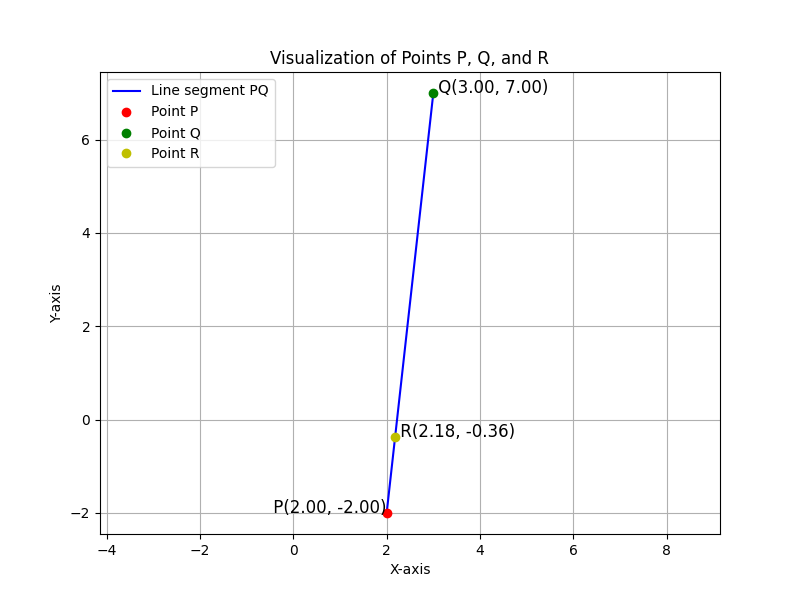
\includegraphics[width=0.7\columnwidth]{figs/1.png}
    \caption{Plot for 1.5.25}
    \label{fig:placeholder}
\end{figure}
\end{frame}
\end{document}